% See exam.cls and examdoc.tex for the license information
\documentclass[12pt, answers]{exam}

\usepackage{amssymb}
\usepackage{makeidx}
\usepackage{amsmath}
\usepackage{graphicx}
\usepackage{caption}
\usepackage{tabulary}
\usepackage{color}
\usepackage{multicol}
\usepackage{multirow}
\usepackage{enumerate}
\usepackage{float}
\usepackage{colortbl}
\usepackage[table,xcdraw]{xcolor}

\usepackage{array}
\newcolumntype{C}[1]{>{\centering\let\newline\\\arraybackslash\hspace{0pt}}m{#1}}

\addpoints

% In case we're not using hyperref.sty:
\providecommand{\texorpdfstring}[2]{#1}
% The following can be used in \section commands
% without generating pdf warnings:
\newcommand{\bs}{\texorpdfstring{\char`\\}{}}

\makeindex

\newcommand{\indc}[1]{\index{#1@\texttt{\char`\\#1}}}
\newcommand{\indcsub}[2]{\index{#1@\texttt{\char`\\#1}!#2}}
\newcommand{\indcstart}[1]{\index{#1@\texttt{\char`\\#1}|(}}
\newcommand{\indcstop}[1]{\index{#1@\texttt{\char`\\#1}|)}}

\newcommand{\indt}[1]{\index{#1@\texttt{#1}}}
\newcommand{\indtsub}[2]{\index{#1@\texttt{#1}!#2}}
\newcommand{\indtstart}[1]{\index{#1@\texttt{#1}|(}}
\newcommand{\indtstop}[1]{\index{#1@\texttt{#1}|)}}

\extraheadheight{-.4in}

\pagestyle{headandfoot}
%\extraheadheight{.2 in}
\firstpageheader{}{}{}
\runningheader{}{}{}
\firstpagefooter{INF281}{Exercise 05}{Page \thepage\ of \numpages}
\firstpagefootrule
\runningfooter{INF281}{Exercise 05}{Page \thepage\ of \numpages}
\runningfootrule

%---------------------------------------------------------------------

\shadedsolutions
%\noprintanswers
\definecolor{SolutionColor}{rgb}{0.8,0.9,1}
\newcommand{\mybox}[1]{\par\noindent\colorbox{SolutionColor}
{\parbox{\dimexpr\textwidth-2\fboxsep\relax}{#1}}}

\begin{document}

\section*{INF281 Exercise 05}

%---------------------------------------------------------------------
\begin{questions}

%%% Question 1
\question \textbf{Non-parametric test}
  
A non-parametric test is used to determine a p-value for the optimal score of a global alignment. Assume we randomly generated 9 sequences and calculated the alignment scores as follows.

\begin{verbatim}
    q: AACG
\end{verbatim}

\begin{table}[H]
\centering
\begin{tabular}{|l|l|l|l|l|l|l|l|l|l|}
\hline
Seq No. & 1   & 2   & 3   & 4   & 5   & 6   & 7   & 8   & 9   \\ \hline
Score   & 0.2 & 0.4 & 0.5 & 1.2 & 1.2 & 1.5 & 1.9 & 2.2 & 2.1 \\ \hline
\end{tabular}
\end{table}

\vspace{0.1 in}

\begin{parts}

%% (a)
  \part What are $H_{0}$ (null hypothesis) and $H_{1}$ (alternative hypothesis) if you want to use a statistical hypothesis test to evaluate a global pairwise alignment in terms of finding homologues?

\begin{solution}[0.35 in]
$H_{0}$:  Sequences are not homologous, $H_{1}$:  Sequences are homologous
\end{solution}

%% (b)
\part Calculate the p-value for the alignment below. 

\begin{verbatim}
    q: AACG
    d: AGTG

    Score: 2
\end{verbatim}
\medskip 

The p-value can be calculated as:

\begin{center}
$p=(b+1)/(n+1)$
\end{center}

where $b$ is the number of randomly generated scores above the score of the original alignment, and $n$ is the sample size. 

\begin{solution}[0.35 in]
p-value:  0.3
\end{solution}

%% (c)
\part Is the test result statistically significant when $\alpha$ = 0.05?

\begin{solution}[0.35 in]
No.
\end{solution}

%% (d)
\part What is the conclusion of the test in terms of finding homologues?

\begin{solution}[0.35 in]
q and d are not homologous.
\end{solution}

\end{parts}


\newpage

%%% Question 2
\question \textbf{Gumbel distribution}
  
Use the alignment scores between q and 5 randomly generated sequences below to answer the following questions.

\begin{verbatim}
    q: ACGTA
\end{verbatim}

\begin{table}[H]
\centering
\begin{tabular}{|l|l|}
\hline
Randomly generated sequence & Alignment score \\ \hline
ACGTA                       & 4               \\ \hline
TTACG                       & 5               \\ \hline
CGCGA                       & 6               \\ \hline
ATTAT                       & 4               \\ \hline
CGATC                       & 6               \\ \hline
\end{tabular}
\end{table}

\vspace{0.1 in}

\begin{parts}

%% (a)
  \part What is the mean of the scores?

\begin{align*}‎
\bar{x} =\dfrac{1}{n} \sum_{i=1}^{n}x_{i}
\end{align*}

\begin{solution}[0.35 in]
5
\end{solution}

%% (b)
\part What is the standard deviation of the scores?

\begin{align*}‎
s = \sqrt{\dfrac{\sum_{i=1}^{n}(x_{i}-\bar{x})^2}{n-1}}
\end{align*}

\begin{solution}[0.35 in]
1
\end{solution}

%% (c)
\part The parameters $\mu$ and $\lambda$ of the Gumbel distribution can be estimated from the mean and the variance of a sample. Calculate  lambda and mu.
\medskip 

\begin{center}
$\mathrm{lamda} \approx \dfrac{1.282}{s}$
\end{center}
\medskip 

\begin{center}
$\mathrm{mu} \approx \bar{x} - \dfrac{0.577}{\mathrm{lamda}}$
\end{center}
\medskip 

\begin{solution}[0.35 in]
lamda: 1.282, mu: 4.55
\end{solution}

%
% NEWPAGE
%
\newpage

%% (d)
\part What is the p-value when the score of an alignment is 4.55?

\begin{table}[H]
\centering
\begin{tabular}{|l|l|}
\hline
x  & exp(x) \\ \hline
0  & 1      \\ \hline
-1 & 0.3679 \\ \hline
-2 & 0.1353 \\ \hline
-3 & 0.0497 \\ \hline
\end{tabular}
\end{table}

$P[Y>4.55]=1-F_Y (4.55)=1 - \exp (-e^{-\lambda(4.55-\mu)})$ \\

\begin{solution}[0.35 in]
$1-0.3679=0.6321$
\end{solution}

%% (e)
\part What is the conclusion of the test in terms of finding homologues?

\begin{solution}[0.35 in]
The sequences of the alignment with score 4.55 are not homologous.
\end{solution}


\end{parts}


\bigskip 

%%% Question 3
\question \textbf{Bit score}
  
BLAST reports bit scores, which are equivalent to the information content that are calculated from raw scores.

\begin{itemize}
\item Bit score: $S' = \dfrac{(\lambda S - \ln⁡ K)}{\ln⁡ 2}$
\item S: raw score
\item K and $\lambda$: Karlin-Altschul statistics
\end{itemize}

\begin{table}[H]
\centering
\begin{tabular}{|l|l|}
\hline
x  & $\ln x$ \\ \hline
1 & 0 \\ \hline
2 & 0.693 \\ \hline
3 & 1.099 \\ \hline
\end{tabular}
\end{table}

Assume K: 3 and $\lambda$: 0.1 and use the table above to answer the following questions.

\vspace{0.1 in}

\begin{parts}

%% (a)
  \part What is the bit score when the raw score is 80.29?

\begin{solution}[0.75 in]
$\dfrac{0.1 \times 80.29 - 1.099}{0.693} = \dfrac{6.93}{0.693} = 10$
\end{solution}

%% (b)
\part $2^{S'}$ indicates the expected search space size that one can find an alignment with score at least S by chance alone. What is the $2^{S'}$ value when the raw score is 17.92?

\begin{solution}[0.75 in]
$S' = \dfrac{0.1 \times 17.92 - 1.099}{0.693} = \dfrac{0.693}{0.693} = 1;$ \quad $2^{1} = 2$
\end{solution}

\end{parts}


\newpage

%%% Question 4
\question \textbf{Bit score to e-value}
  
The e-value represents the expected number of hits when homologous sequence are searched on a database of a particular size. It can be calculated from a bit score as follows. 
 
 $E = \dfrac{\mathrm{Size \, of \, search \, space}}{2^{\mathrm{bit-score}}}$

\vspace{0.1 in}

\begin{parts}

%% (a)
  \part What is the e-value when the size of search space is 3200 and the bit score is 4?

\begin{solution}[0.75 in]
$\dfrac{3200}{2^4} = \dfrac{3200}{16} = 200$
\end{solution}

%% (b)
\part Assume we can calculate a search space size as $m \times n$ where $m$ is the query sequence size and $n$ is the total character size of a database. What is the e-value when $m$ is 20, $n$ is 4000, and the bit score is 3?

\begin{solution}[0.75 in]
$\dfrac{20 \times 4000}{2^3} = \dfrac{80000}{8} = 10000$
\end{solution}

\end{parts}


\bigskip 

%%% Question 6
\question \textbf{Raw score to e-value}
 The e-value can be directly caudated from a raw score as $E(S)=Kmne^{-\lambda S}$. Use the values below to answer the following questions.

\begin{itemize}
\item K: 2
\item $\lambda$: 0.1
\end{itemize}

\begin{table}[H]
\centering
\begin{tabular}{|l|l|}
\hline
x  & exp(x) \\ \hline
0  & 1      \\ \hline
-1 & 0.3679 \\ \hline
-10 & 0.000045 \\ \hline
\end{tabular}
\end{table}

\vspace{0.1 in}

\begin{parts}

%% (a)
  \part What is E(10) when m is 10 and n is 100?

\begin{solution}[0.35 in]
$E(10)=2 × 10 × 100 × e^{-1}=7358$
\end{solution}

%% (b)
\part What is E(100) when m is 10 and n is 100?

\begin{solution}[0.35 in]
$E(100)=2 × 10 × 100 × e^{-10}=0.09$
\end{solution}

%% (c)
\part What is E(100) when m is 100 and n is 1000?

\begin{solution}[0.35 in]
$E(100)=2 × 100 × 1000 × e^{-10}=9$
\end{solution}

\end{parts}


\newpage

%%% Question 7
\question \textbf{Basic measures from confusion matrix}
  
The oval representation below shows that a model has classified a test data set with 10 positives and 10 negatives and produced four outcomes.
 
\begin{figure}[H]
      \centering
      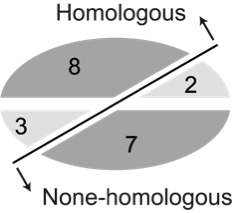
\includegraphics[width=0.2 \textwidth]{fig07/oval_representation.png}
\end{figure}

\vspace{0.1 in}

\begin{parts}

%% (a)
  \part Fill each blank cell with one of the four classification outcomes - TP, FP, TN, and FN.

\begin{table}[H]
\centering
\begin{tabular}{ll|c|c|}
\cline{3-4}
                                                             &                & \multicolumn{2}{c|}{Test data}                                        \\ \cline{3-4} 
                                                             &                & \multicolumn{1}{l|}{Homologous} & \multicolumn{1}{l|}{Non-homologous} \\ \hline
\multicolumn{1}{|l|}{}                                       & Homologous     & \cellcolor[HTML]{CCE5FF}TP      & \cellcolor[HTML]{CCE5FF}FP          \\ \cline{2-4} 
\multicolumn{1}{|l|}{\multirow{-2}{*}{Model classification}} & Non-homologous & \cellcolor[HTML]{CCE5FF}FN      & \cellcolor[HTML]{CCE5FF}TN          \\ \hline
\end{tabular}
\end{table}

%% (b)
\part Make a confusion matrix for the oval representation.

\begin{table}[H]
\centering
\begin{tabular}{ll|c|c|}
\cline{3-4}
                                                             &                & \multicolumn{2}{c|}{Test data}                                        \\ \cline{3-4} 
                                                             &                & \multicolumn{1}{l|}{Homologous} & \multicolumn{1}{l|}{Non-homologous} \\ \hline
\multicolumn{1}{|l|}{}                                       & Homologous     & \cellcolor[HTML]{CCE5FF}8      & \cellcolor[HTML]{CCE5FF}3          \\ \cline{2-4} 
\multicolumn{1}{|l|}{\multirow{-2}{*}{Model classification}} & Non-homologous & \cellcolor[HTML]{CCE5FF}2      & \cellcolor[HTML]{CCE5FF}7          \\ \hline
\end{tabular}
\end{table}

%% (c)
  \part Calculate the following basic evaluation measures for the oval representation. Round off the answer to two decimal places if necessary.

\bigskip 
Accuracy
$= \dfrac{TP+TN}{P+N} $ \colorbox{SolutionColor}{$= \dfrac{15}{20} = 0.75$}

\bigskip 
Error rate
$= \dfrac{FP+FN}{P+N} $ \colorbox{SolutionColor}{$= \dfrac{5}{20} = 0.25$}

\bigskip 
Sensitivity
$= \dfrac{TP}{P} $ \colorbox{SolutionColor}{$= \dfrac{8}{10} = 0.8$}

\bigskip 
Specificity
$= \dfrac{TN}{N} $ \colorbox{SolutionColor}{$= \dfrac{7}{10} = 0.7$}

\bigskip 
Precision
$=\dfrac{TP}{TP+FP}$ \colorbox{SolutionColor}{$= \dfrac{8}{11} = 0.73$}

\end{parts}



%%% Question 8
\question \textbf{Measures with multiple thresholds}
  
Create multiple confusion matrices by considering all possible threshold values. Assume that the test data set contains two positives and two negatives. The table below shows the scores given by a model that gives higher scores for the alignments with higher similarities. 

\begin{table}[H]
\centering
\begin{tabular}{|l|l|l|l|l|}
\hline
Test set label & P   & P   & N   & N   \\ \hline
Model score    & 2.1 & 3.1 & 2.3 & 1.2 \\ \hline
\end{tabular}
\end{table}

\vspace{0.1 in}

\begin{parts}

%% (a)
  \part Fill the labels that match the sorted scores

\begin{figure}[H]
      \centering
      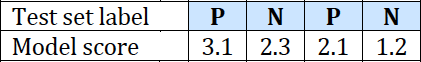
\includegraphics[width=0.4 \textwidth]{fig07/sorted_test_solution.png}
\end{figure}


%% (b)
\part Fill the labels predicted by different threshold values.

\begin{figure}[H]
      \centering
      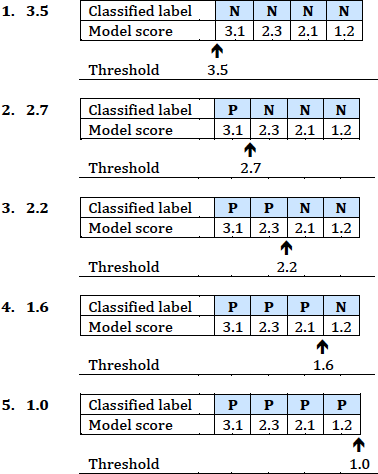
\includegraphics[width=0.6 \textwidth]{fig07/thresholds_solution.png}
\end{figure}

%
% NEWPAGE
%
\newpage

%% (c)
  \part Use the labels in (a) and (b) and calculate TP, FP, TN, and FN for all threshold values.

\begin{table}[H]
\centering
\begin{tabular}{|l|c|c|c|c|}
\hline
Threshold & \multicolumn{1}{l|}{TP}   & \multicolumn{1}{l|}{FP}   & \multicolumn{1}{l|}{TN}   & \multicolumn{1}{l|}{FN}   \\ \hline
3.5       & \cellcolor[HTML]{CCE5FF}0 & \cellcolor[HTML]{CCE5FF}0 & \cellcolor[HTML]{CCE5FF}2 & \cellcolor[HTML]{CCE5FF}2 \\ \hline
2.7       & \cellcolor[HTML]{CCE5FF}1 & \cellcolor[HTML]{CCE5FF}0 & \cellcolor[HTML]{CCE5FF}2 & \cellcolor[HTML]{CCE5FF}1 \\ \hline
2.2       & \cellcolor[HTML]{CCE5FF}1 & \cellcolor[HTML]{CCE5FF}1 & \cellcolor[HTML]{CCE5FF}1 & \cellcolor[HTML]{CCE5FF}1 \\ \hline
1.6       & \cellcolor[HTML]{CCE5FF}2 & \cellcolor[HTML]{CCE5FF}1 & \cellcolor[HTML]{CCE5FF}1 & \cellcolor[HTML]{CCE5FF}0 \\ \hline
1         & \cellcolor[HTML]{CCE5FF}2 & \cellcolor[HTML]{CCE5FF}2 & \cellcolor[HTML]{CCE5FF}0 & \cellcolor[HTML]{CCE5FF}0 \\ \hline
\end{tabular}
\end{table}

%% (d)
  \part Use the result in (c) and calculate basic evaluation measures. Round off the answer to one decimal place if necessary.

\begin{table}[H]
\centering
\begin{tabular}{|l|c|c|c|}
\hline
Threshold & \multicolumn{1}{l|}{Specificity} & \multicolumn{1}{l|}{1 - specificity} & \multicolumn{1}{l|}{Sensitivity} \\ \hline
3.5       & \cellcolor[HTML]{CCE5FF}1        & \cellcolor[HTML]{CCE5FF}0            & \cellcolor[HTML]{CCE5FF}0        \\ \hline
2.7       & \cellcolor[HTML]{CCE5FF}1      & \cellcolor[HTML]{CCE5FF}0          & \cellcolor[HTML]{CCE5FF}0.5      \\ \hline
2.2       & \cellcolor[HTML]{CCE5FF}0.5      & \cellcolor[HTML]{CCE5FF}0.5          & \cellcolor[HTML]{CCE5FF}0.5      \\ \hline
1.6       & \cellcolor[HTML]{CCE5FF}0.5       & \cellcolor[HTML]{CCE5FF}0.5            & \cellcolor[HTML]{CCE5FF}1        \\ \hline
1         & \cellcolor[HTML]{CCE5FF}0        & \cellcolor[HTML]{CCE5FF}1            & \cellcolor[HTML]{CCE5FF}1        \\ \hline
\end{tabular}
\end{table}

%% (e)
  \part Draw a ROC curve for the calculated evaluation measures in (d).

\begin{figure}[H]
      \centering
      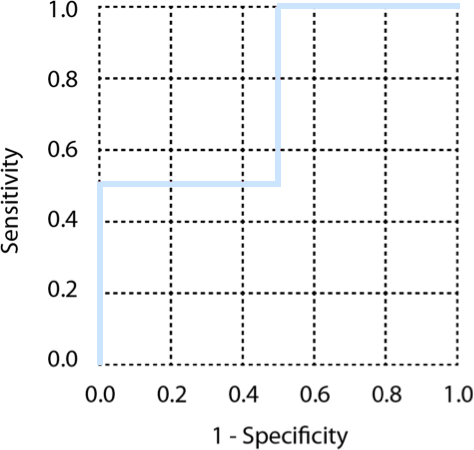
\includegraphics[width=0.3 \textwidth]{fig07/roc_sol.png}
\end{figure}

%% (f)
  \part Calculate the area under the curve of the curve in (e).
  
\begin{solution}[0.35 in]
0.75
\end{solution}

%% (g)
  \part Evaluate the ROC curve in your own words.
  
\begin{solution}[0.35 in]
The model performs better than random classifiers
\end{solution}

\end{parts}



\end{questions}
%---------------------------------------------------------------------
       
\end{document}

